%%%%%%%%%%%%%%%%%%%%%%%%%%%%%%%%%%%%%%%%%%%%%%%%%%%%%%%%%%%%%%%%%%%%%%%%%%%%%%%%
%2345678901234567890123456789012345678901234567890123456789012345678901234567890
%        1         2         3         4         5         6         7         8
\documentclass[letterpaper, 10 pt, conference]{ieeeconf}  % Comment this line out if you need a4paper
\IEEEoverridecommandlockouts                              % This command is only needed if 
                                                         % you want to use the \thanks command
\usepackage[utf8]{inputenc}
\usepackage{amsmath}
\usepackage{bm}
\usepackage{amssymb}
\usepackage{graphicx}
\usepackage{booktabs}
\usepackage{mathrsfs}
\usepackage{amsbsy}
\usepackage{caption}
\usepackage{float}
\usepackage{subcaption}
\usepackage{varwidth}
\usepackage{algorithm}
\usepackage{tabularx}
\usepackage{yhmath}
\usepackage{multirow}
\usepackage{multicol}
\usepackage{booktabs}
\usepackage{rotating}
\usepackage[table]{xcolor}
\definecolor{grey}{rgb}{0.9,0.9,0.9}
\usepackage[noend]{algpseudocode}
\usepackage[top=60pt,left=48pt,right=48pt,bottom=45pt]{geometry}	
\usepackage{dsfont}
\usepackage{environ}
\usepackage[framemethod=TikZ]{mdframed}
\usepackage{algorithm}
\usepackage{accents}\newcommand\addtag{\refstepcounter{equation}\tag{\theequation}}
\usepackage{etoolbox}
\usepackage{graphicx}
\usepackage{rotating}
\usepackage{enumerate}
\usepackage[colorlinks]{hyperref}
\usepackage{relsize}
\usepackage{gensymb}
\usepackage{cleveref}
\usepackage{threeparttable}
\usepackage{colortbl}
\definecolor{Gray}{gray}{0.9}
\newcommand{\comFB}[1]{\noindent\colorbox{yellow}{\parbox{\dimexpr\columnwidth-1\fboxsep}{[FB: #1]}}}
%%% Customized commands
%%% math commands
\newcommand{\mvec}[1]{\bm{#1}}
\newcommand{\dmvec}[1]{\dot{\mvec{{#1}}}}
\newcommand{\ddmvec}[1]{\ddot{\mvec{{#1}}}}

\newcommand{\xt}{\mvec{x}(t)}
\newcommand{\ut}{\mvec{u}(t)}

\newcommand{\st}{\text{s.t.}}
\newcommand{\g}{\mvec{g}}
\newcommand{\q}{\mvec{q}}
\newcommand{\dq}{\dmvec{q}}
\newcommand{\ddq}{\ddmvec{q}} 

%%% table commands
\newcommand{\mymultirow}[2]{\parbox[t]{2mm}{\multirow{#1}{*}{\rotatebox[origin=c]{90}{#2}}}}
%%% Document
\title{\LARGE \bf Bioptim, a Python interface for Musculoskeletal Optimal Control in Biomechanics}
\author{author$\#1$\textsuperscript{a,*}, author$\#2$\textsuperscript{a}, author$\#3$\textsuperscript{b}  and  author$\#4$\textsuperscript{a}% <-this % stops a space
\thanks{\textsuperscript{a}\,Laboratoire de Simulation et Modélisation du Mouvement, Faculté de Médecine, Université de Montréal, Laval, QC, Canada}%
\thanks{\textsuperscript{b}\,other, elsewhere}%
\thanks{\textsuperscript{*}\,author$\#1$@umontreal.ca}
}

%%% User commands

\usepackage{pdfrender}
\DeclareRobustCommand*{\pmbb}[1]{%
  \textpdfrender{
    TextRenderingMode=Stroke,
    LineWidth=.1pt,
  }{#1}%
}
\NewEnviron{comeq}{%
\par\vspace{0ex}
\begin{mdframed}[outerlinewidth=0.5,leftmargin=10,rightmargin=-10pt,backgroundcolor=white,hidealllines=true,leftline=true,
innertopmargin=0pt,splittopskip=0, skipbelow=\baselineskip, innerbottommargin=0pt%
skipabove=0ex]%
\vspace{-0ex}\hspace{0pt}\textit{Proof:}%
\itshape
\begin{equation*} 
\begin{split}
\BODY
\end{split}
\end{equation*}
\end{mdframed}
}
\newcommand{\pd}[2]{\frac{\partial #1}{\partial #2}}
\def\abs{\operatorname{abs}}
\def\argmax{\operatornamewithlimits{arg\,max}}
\def\argmin{\operatornamewithlimits{arg\,min}}
\def\diag{\operatorname{Diag}}
\newcommand{\eqRef}[1]{(\ref{#1})}
\newcommand{\dbtilde}[1]{\accentset{\approx}{#1}}

\hyphenpenalty=10000

\begin{document}

\maketitle
\thispagestyle{plain}
\pagestyle{plain}

\begin{abstract}
Musculoskeletal simulations are useful in biomechanics to investigate the causes of movement disorder, to estimate non-measurable physiological quantities or to study the optimality of human movement.
We introduce \bioptim, an easy-to-use Python framework for biomechanical optimal control, handling musculoskeletal models. 
Relying on algorithmic differentiation and the multiple shooting formulation, \bioptim interfaces nonlinear solvers to quickly provide dynamically consistent optimal solutions.
The software is both computationally efficient (C++ core) and easily customizable, thanks to its Python interface.
It allows to quickly define a variety of biomechanical problems such as motion tracking/prediction, muscle-driven simulations, parameters optimization, multiphase problems, etc.
It is also intended for real-time applications such as moving horizon estimation and model predictive control.
Six contrasting examples are presented, comprising various models, dynamics, objective functions and constraints. 
They include data-driven simulations (i.e., a multiphase muscle driven gait cycle and an upper-limb real-time moving horizon estimation of muscle forces) and predictive simulations (i.e., a muscle-driven pointing task, a twisting somersault with a quaternion-based model, a position controller using external forces, and a multiphase torque-driven maximum-height jump motion).
\end{abstract}

\textbf{Keywords -- Biomechanics, Optimization, Optimal control, Musculoskeletal simulation, Software}



\section{Introduction}\label{sec:introduction}
Biomechanics researchers rely on numerical simulations of motion to gain understanding on a variety of scientific topics such as the physiological causes of movement disorders and their consequences on health [\addref], the estimation of non-measurable physiological quantities (e.g., muscle forces)[\addref] and the optimality of human movement [\addref].
The musculoskeletal models used in these simulations generally have a large number of degrees of freedom and they are governed by several ordinary differential equations (ODEs) which mainly describe multibody and muscle activation dynamics.
The complexity of these systems has led scientists to formulate their simulations as optimal control problems (OCP), relying on efficient non-linear optimization software to find trajectories that fulfill a desired task while enforcing the system dynamics and minimizing a cost (e.g. motion duration, energy expenditure, matching experimental data, etc.).
Up to very recently, there was no off-the-shelf software available to the community to quickly formulate and solve such musculoskeletal OCPs. 
Consequently, researchers had to develop their own solutions, with little or no dissemination to the community, limiting  synergies between researchers.


As a result, many approaches coexist to formulate and solve OCPs in the biomechanical literature. 
The formulation, also called discretization, consists in turning a continuous trajectory optimization problem into a generic discrete non-linear program (NLP) that is solved using a dedicated algorithm. 
The main family of so-called \textit{direct} transcription methods comes from numerical optimal control. 
They consist in straightforwardly choosing the state and/or the control as optimization variables at a given number of points along the trajectory and they rely on the integration of the system dynamics between these points. 

For instance, the \textit{direct collocation} method has shown its efficiency in some studies investigating human motion [\addref\comment{, \`a prendre dans papier MOCO}{Sinon j'en ai un paquet dans mon Zotero que j'avais fait pour ma préparation de synthèse}]. 
It consists in approximating the integration of the system dynamics using polynomials that describe the state and control trajectories.
Its main advantages are that it leads to very sparse NLPs, that knowledge about the state trajectory can be used in the initialization, and that it handles unstable systems well \cite{diehl2006fast}. 
Its major disadvantage is that adaptive integration error control implies regridding the whole problem and thus changes the NLP dimensions, discarding its use for such application [\addref].
\textit{Direct multiple shooting} is another direct method that was also applied with success in a lot of biomechanics [\addref] and robotics [\addref] studies.
Its advantages are mostly the same as for direct collocation in addition to combine integration error control with fixed NLP dimensions, as it relies on possibly adaptive ODE solvers to integrate the system dynamics.
Besides direct methods, other choices can be made, as in \cite{yeadon2000mechanics} [+ \addref\ Begon], where the optimization variables are instants at which a switch in the motor strategy occurs, using polynomials function (4th, 5th order) in-between, or in \cite{leboeuf2006energetic} [+ \addref\  Huchez, Mombaur, McPhee, Opensim]], where the optimization variables are the coefficients of fourth order polynomial approximations of the states, with linking conditions to enforce the continuity of the controls. 
These last approaches are less generic than the direct methods as they either require a prior knowledge about the state and control trajectories. 
Most of the time, when investigating complex biomechanics issues, we do not have this information. 


\begin{figure}[t!]
\centering
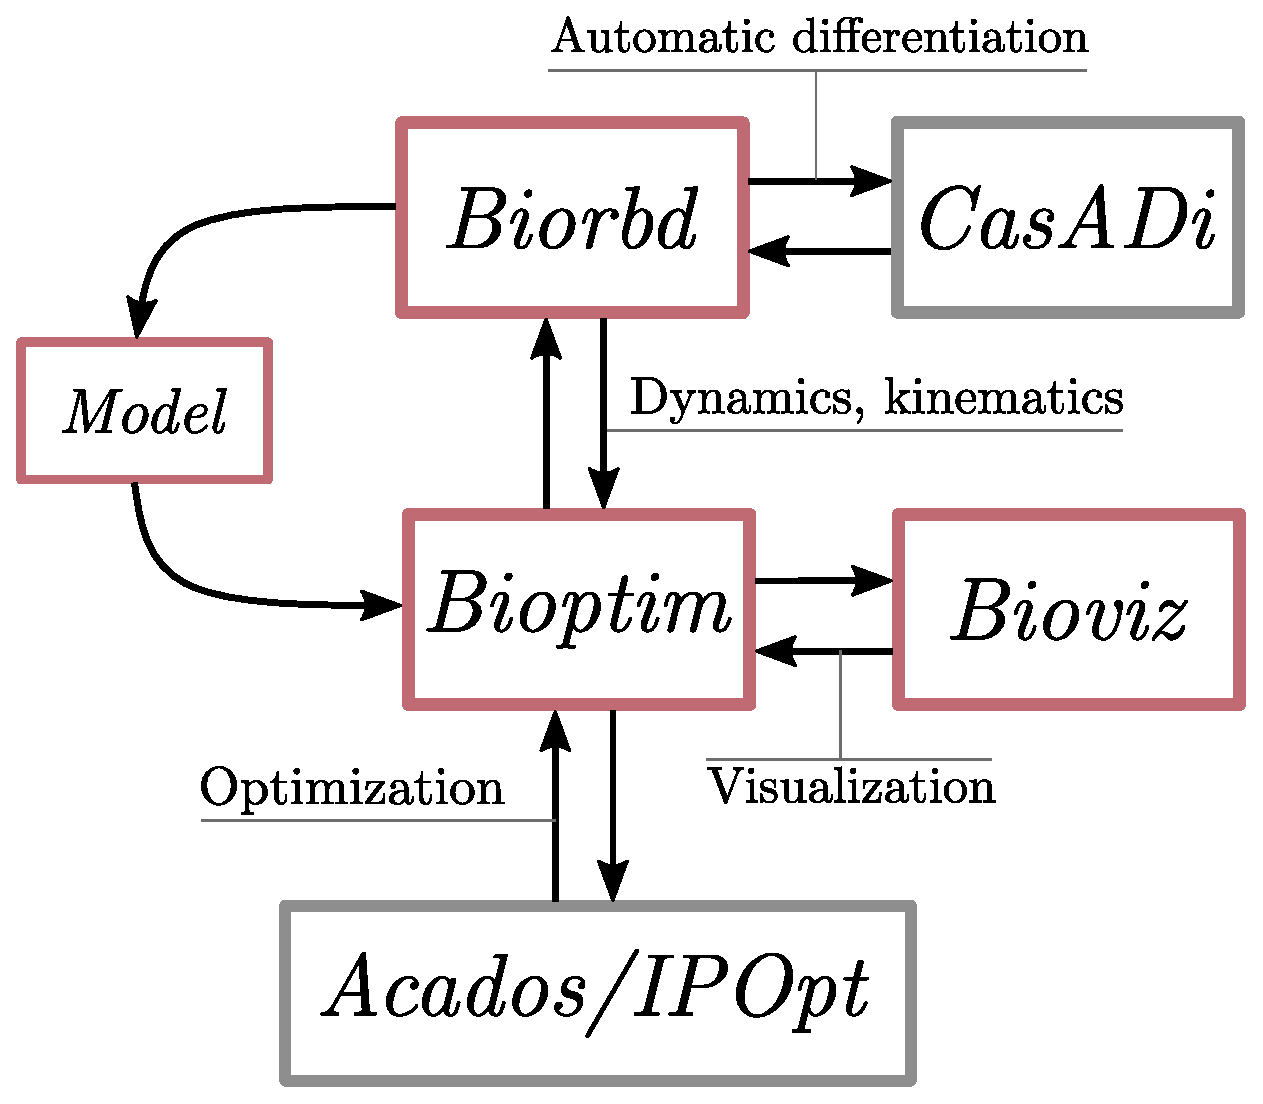
\includegraphics[width=0.9\columnwidth]{figures/dependencies.eps}
\caption{\bioptim dependencies flowchart. The red-boxed software are developed by the S2M team. The \bioptim part is further detailed in Fig.~\ref{fig:dependencies}.}
\label{fig:dependencies}
\vspace*{-0.5cm}
\end{figure}

Concerning the non-linear solver, a variety of software exist and have been used to solve transcribed musculoskeletal NLPs.
They can use different heuristics: interior point methods (\ipopt, [\addref]) or sequential quadratic programming (\textit{snopt} [\addref], \acados [\addref]), but they are all gradient based.
Therefore, derivatives of the NLP cost function and constraints are required to perform optimization.
These derivatives can be obtained by finite differences (often implemented but inaccurate thus comprising convergence) or computed exactly using automatic differentiation (requiring to write all dependencies of the software in symbolic variables) [CasADi].


In order to promote the use of musculoskeletal optimal control among biomechanics researcher, we identified a strong need for a dedicated tool, as shown by the recently launched \moco [\addref, Opensim]. 
The biomechanics community being mainly composed of software users [\addref], such a tool should request a flexible user interface written in a widely used high-level and if possible open-source language (e.g. Python) with a low-level core (e.g. C++) for efficiency. 

To develop such a software, four interrelated components are essential to us: \textit{i)} a musculoskeletal modeling software, with a visualization module (multibody kinematics and dynamics, muscle dynamics, etc.), \textit{ii)} a method for automatic differentiation, \textit{iii)} a discretization approach, and \textit{iv)} one or several nonlinear programming (NLP) solvers. 
General-purpose optimal control software (e.g. \gpopsii [\addref], \muscodii [\addref], \acado [\addref]) address \textit{ii)} to \textit{iv)} but they need to be interfaced with a musculoskeletal modeling module and they do not provide any built-in biomechanics features (physiological cost functions, kinematic constraints, etc.). 
In that sense, the aforementioned \moco, is a welcome initiative that draws its strength from its integration with the widely used \opensim.
However, it faces the following limitations: it uses finite differences to avoid the complexity of adapting the \opensim codebase to support automatic differentiation, it uses direct collocation as transcription method, preventing the use of adaptive ODE solvers and it is not as flexible as required by the community, since it requires the user to develop new features, such as new objective functions, in C++. 

The objective of the present paper is to introduce \bioptim, an open-source optimal control software dedicated to musculoskeletal biomechanics.
\bioptim is based on C++ code for computational efficiency but the user interface is written in Python for flexibility and ease-of-use. 
The OCP transcription uses direct multiple shooting to preserve the possibility of using arbitrarily accurate ODE solvers for the integration, which is fully parallelized for more efficiency.
\textit{Bioptim's} core is fully written in \casadi symbolics to benefit from algorithmic differentiation and to exploit \casadi 's interface with several non-linear solvers (\textit{ipopt, snopt}).
Moreover, \bioptim is interfaced with the cutting-edge solver \textit{acados}, a recent NLP solver dedicated to direct multiple shooting, intended for real-time applications.
The purpose of \bioptim is to allow fast and flexible musculoskeletal OCP formulation and solving by providing a framework with a lot of typical biomechanics problem already implemented and customizable.

The paper is organized as follows: first, the design and implementation of \bioptim are described.
Next, the versatility and performances of \bioptim are shown through a variety of examples available online. 


\section{Implementation and Design}\label{sec:design&impl}
\subsection{Implementation and dependencies}
\bioptim is the top layer of a series of libraries (\biorbd: dynamics and MSK modeling; \casadi: automatic differentiation; \ipopt/\acados: optimization; \bioviz: visualization).
Within this software suite, \bioptim 's main role is to shape the problem to allow its dependencies to communicate efficiently, while providing an intuitive and flexible interface to the user (Fig.~\ref{fig:dependencies}).
Therefore, it was written in Python for its flexibility and its widespread use among researchers.
However, all intensive calculations behind the interface are performed in C/C++, keeping \bioptim both fast and easy to customize.

\begin{figure}[t!]
\centering
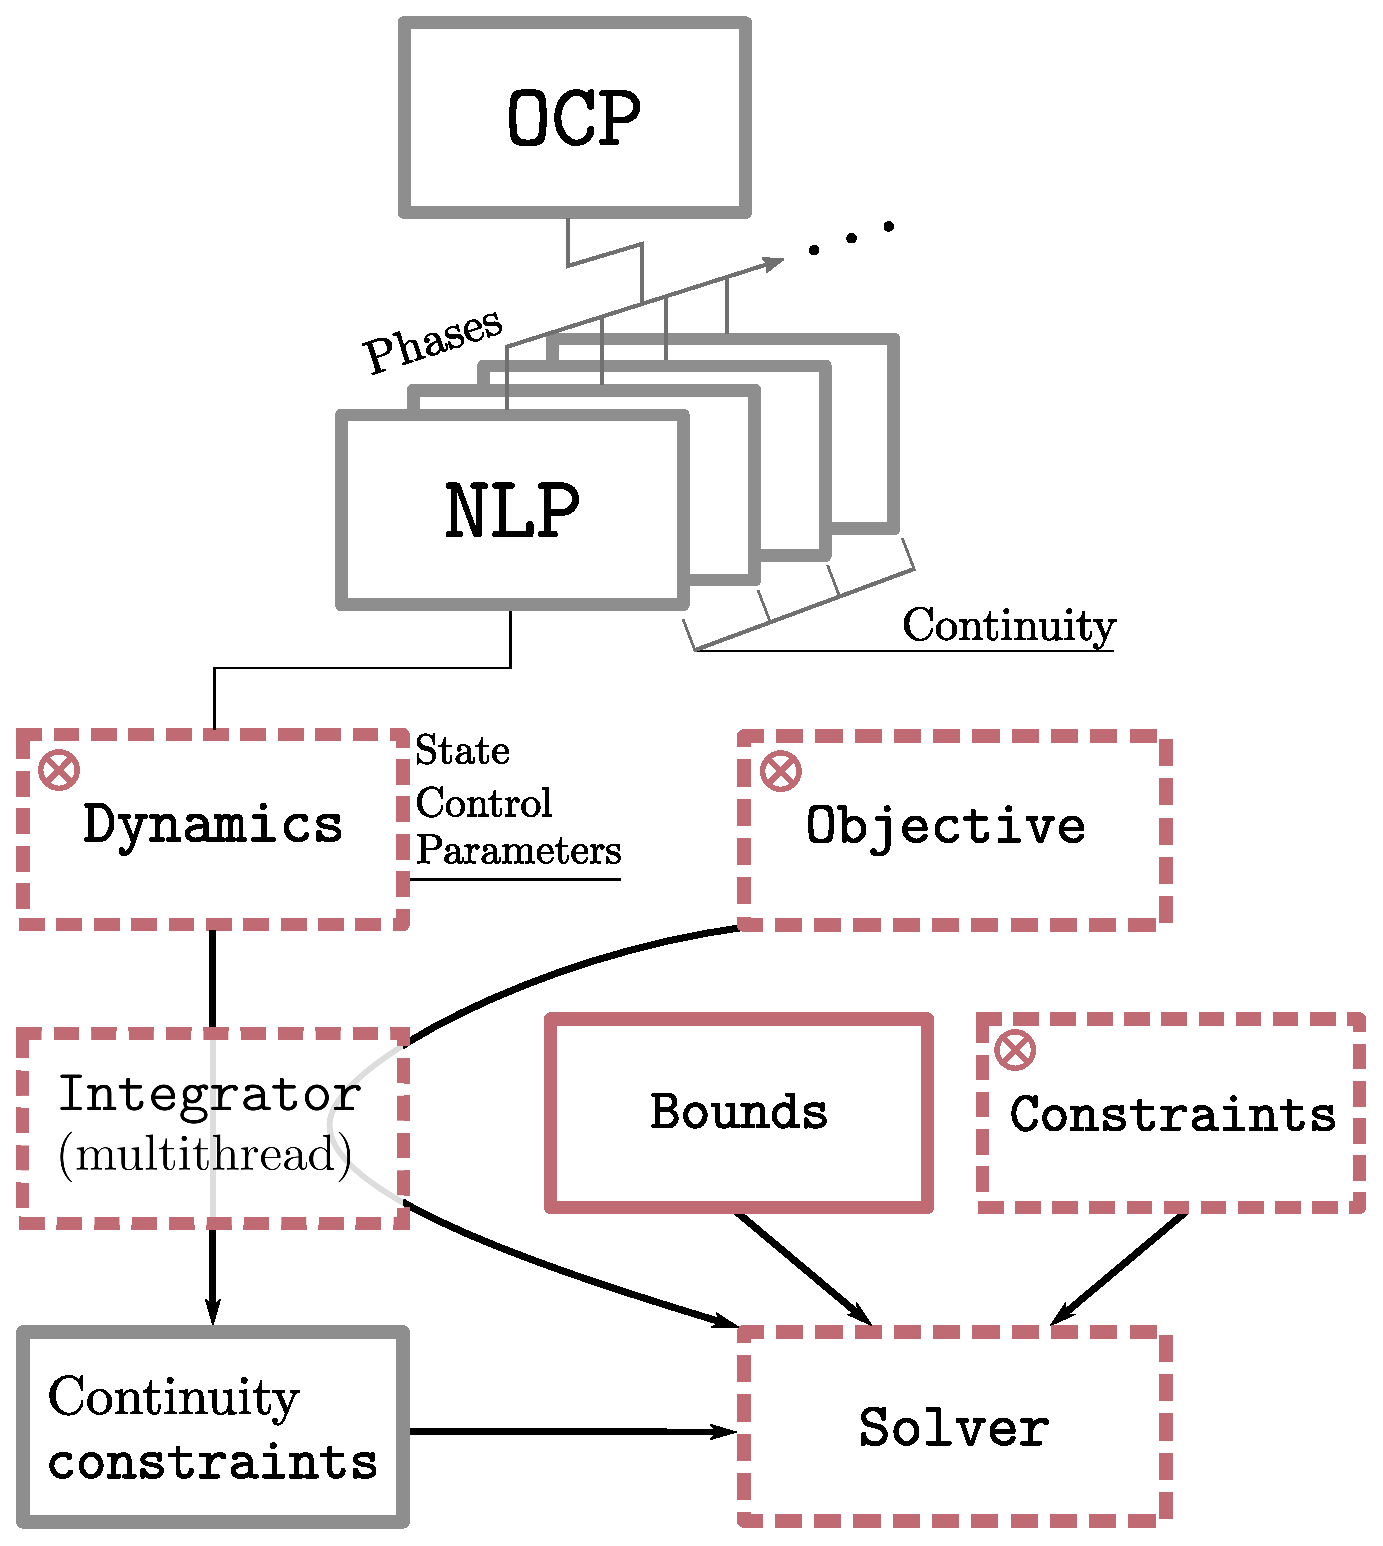
\includegraphics[width=0.9\columnwidth]{figures/design.eps}
\caption{\bioptim design flowchart. The red box correspond to objects that must be filled in by the user. The red-dashed boxes correspond to pre-implemented objects already available to the users. The * stands for easily customizable objects.}
\label{fig:flowchart}
\vspace*{-0.5cm}
\end{figure}


\subsection{Design}
\bioptim shapes and solves optimal control problems whose two required entries are a model (.\textit{bioMod} file) and an OCP.
The model file contains the geometrical characteristics and the segment inertial parameters as well as optional elements, namely, the markers, the actuators of the model (muscles and joint torques possibly with torque/angle/velocity relationships) as well as bounds on joint kinematics and torques. 
It also allows the user to design or import meshes for visualization purposes.
The \texttt{OCP} consists in a combination of nonlinear problems (NLPs) that allows for the formulation of multi-staged OCPs. 
Each \texttt{NLP} has the following attributes: \textit{1)} a dynamics type, \textit{2)} an objective function set, \textit{3)} a constraint set, \textit{4)} variables bounds, \textit{5)} a number of shooting points and the duration of the problem and \textit{6)} initial guesses.
Based on these inputs, \bioptim properly sets up the multiple shooting transcription of the OCP, with appropriate continuity constraints (between the shooting nodes and the phases) and shapes it up to feed the chosen nonlinear solver (\ipopt or \acados). 
Next, we develop the different attributes of each \texttt{NLP}:

\subsubsection{Dynamics}
The dynamics defines which variables are states ($\state$), controls ($\control$) and parameters ($\param$), the latter being time-independent.
Then, it implements the ordinary differential equation governing the state dynamics:

\[
\dstate = f(\state, \control, \param).
\addtag
\label{eq:state_transition}
\]

\noindent More than 10 dynamics are already implemented in \bioptim \footnote{\href{https://github.com/pyomeca/bioptim/blob/master/bioptim/dynamics/dynamics_functions.py}{github link}}, among which the controls can be muscle excitations, muscle activations and/or joint torques, the states can be muscle activations and/or joint kinematics.
They can include contact points, external forces, etc.
Even if these dynamics types exhaustively span the current usages in biomechanics, a custom dynamics type is also pre-implemented to easily customize problems.

\subsubsection{Objective function set}
In line with the optimal control formalism, there are two main types of objective functions, namely Lagrange and Mayer. 
Lagrange types are running objectives, integrated over the NLP duration. Mayer types are time-specific objectives. 
Classically, they correspond to a terminal objective, but to be more versatile, they can be defined at any instant in \bioptim.

Objective functions can depend on any of the optimization variable, \textit{i.e.} the controls, the states, the parameters and the duration of the problem. 
A lot of objective function types are already implemented in \bioptim ($>\!20$), among which tracking\:/\:minimizing, on states\:/\:controls\:/\:markers\:/\:contact\:forces\:/\:problem\:duration, etc. 
Should one go missing, a custom objective type is also possible to define.

When declaring the desired list of objective functions for a given NLP, each objective function type is associated with a weight, and the user can choose on which components of the vector variables the objective must apply. 
If applicable (for tracking objective functions mainly), the user must also specify the numerical target of the objective.

\subsubsection{Constraint set}
Classically, constraints are hard penalties of the optimization problem, i.e., a solution will not be considered optimal, unless all constraints (equality or inequality) are met.
The \texttt{Constraint} class contains a variety of already implemented constraints.
Some of them are specific functions, commonly useful in biomechanical problems (e.g. non-slipping contact point, non-linear bounds on torque depending on the state, etc.), the others have their equivalent in the \texttt{ObjectiveFunction} class.
Should one go missing, a custom constraint type is also possible to define.

\subsubsection{Bounds}
Essentially, the \texttt{Bounds} are constraints directly related to the states, the controls and the parameters.
They are useful for defining model-related constraints such as kinematic, torque or muscle excitation\:/\:activation limits. 

\subsubsection{Shooting points and problem duration}
In a direct multiple shooting formulation, the total duration of the problem is divided into smaller intervals whose initial values are called shooting points. 
In \bioptim, the user is asked to define a number of shooting points and a problem duration, per phase.
Possibly, the problem duration can be part of the optimization variables, allowing for, e.g., minimal time formulations.

\subsubsection{Initial guesses}
Once the problem is set up, the user can provide an \texttt{InitialGuess} for all the optimization variables, at each shooting point.
This feature aims at providing prior information to the solver.
Several \texttt{InterpolationTypes} are implemented in \bioptim (constant, linear, spline, each shooting point, etc.), to quickly let the user define the initial guesses.
A custom \texttt{InterpolationType} is also possible to implement.

\section{Examples}\label{sec:Examples}
\include{sections/Examples}

\section{Discussion}\label{sec:discussion}
The purpose of \textit{bioptim} is to solve a variety of biomechanical OCPs with minimal user effort and high performances in terms of computational time. 
The main features illustrated by the six provided examples are (Tab.~X): 
\textit{i)} the possibility to use torque-, activation- or excitation-driven models (and their combinations);
\textit{ii)} a variety of ready-to-use cost functions, constraints and dynamics (with and without contacts)...;
\textit{iii)} ... easily customizable in Python when required by the user;
\textit{iv)} the possibility to solve advanced OCPs (possibly multi-phased) in a few seconds or minutes, that were previously known to take hours; 
\textit{v)} the interface with two different NLP solvers.
In the following, several aspects of \textit{bioptim} are discussed.

\subsection{Direct multiple shooting-based}

While the debate remains about the performances of direct collocations versus DMS \cite{diehl2006fast}\hl{[donner d'autres favorables a DC]}, the development of \textit{bioptim} was oriented toward DMS, because: \textit{i)} it allows to select effortlessly an arbitrary accuracy for the integration (e.g., number of RK steps); \textit{ii)} it allows to use DMS-based fast NLP solvers such as \textit{acados}.
Concerning the integration, either internally or via \textit{acados}, several schemes are implemented in \textit{bioptim} (RK4, RK8, IRK).
While IRK showed better convergence in our experience with hard problems in \textit{acados}, in most of the cases, RK4 showed to be a good speed/robustness trade-off. 
In contrast to what is claimed in several papers [\addref], DMS is not a limitation to the performances (cost value and time to convergence), since the performances of \textit{bioptim} often outperform state-of-the-art results.

\subsection{Automatic differentiation}

One of the reasons explaining the performances of \textit{bioptim} is the rewriting of the core software, \textit{RBDL} and \textit{biorbd} implementing the dynamics, into \textit{casadi} symbolics for automatically providing the exact Jacobians and Hessians of the resulting NLP.  
This feature is somewhat more computationally expensive than finite differences, but the gain in precision for the calculation of derivatives often leads to shorter convergence times (due to much less iterations) and to optimal solutions reached with lower tolerances.
This last aspect must be emphasized for complex motions (fast, highly dynamics ones), because talking about \textit{ipopt} for instance, an optimal solution obtained with a convergence criterion of $1e-2$ is very unlikely to be dynamically consistent (it would diverge when forward integrating the controls in a single-shooting manner), whereas a lower tolerance ($1e-6$. $1e-8$) only reachable with exact derivatives could lead to better forward dynamics results.

\subsection{Python based but fast!}

\textit{bioptim} was thought as an interface, and was therefore written in Python to allow the user to easily combine existing cost functions or constraints and self-implemented ones, to switch from one solver to another, etc. 
We believe this feature to be of importance given that the biomechanics community is known to be mainly made of software users rather than developers.
Therefore, providing a custom interface in Python rather than in, e.g., C++ [MOCO], was a driving objective of our work.
But since flexibility and ease-of-use should not compromise the performances, all the inside computations are expressed as C++ CasAdi graphs, interfaced with C++ NLP solvers.
These graphs can either be built in \texttt{casadi.MX()} or \texttt{casadi.SX()}.
\textit{acados} requires the latter, needing more RAM for building the problem but being faster to solve, whereas both options are available when using \textit{ipopt}. 
Inspired by the  real-time graphics from \textit{MUSCOD-II} \hl{[ref]}, \textit{bioptim} proposes a series of online-generated figures to analyze the iterations of the solvers with  minimal computational cost thanks to a \hl{XXX} protocole. 
Our implementation leverages the \textit{Python pickle} library for easily saving and loading OCPs for, e.g., post-processing analysis.

\subsection{Fast vs robust NLP solvers}

Fast solvers, such as \textit{acados}, offer the opportunity to use multi-start approaches on complex problems in order to circumvent the obstacle of local minima \cite{huchez2015local, bailly2020optimal} or to get meaningful initial solutions from simpler problems, for guiding the resolution of the harder problems.
On the other hands, robust solvers, such as \textit{ipopt}, are convenient when the user lacks information about the sought solutions and thus cannot guide the solver through a good initial guess.
For biomechanics applications, the complementary characteristics of the interfaced solvers is a really useful tool.

\subsection{Multiphase}

Biomechanics studies often face changing dynamics due to the loss or gain of contact or \hl{XXX}.
When tracking such a motion or trying to predict it, these dynamics changes translate into multi-phase OCP.
This is currently one of the drawbacks of \textit{moco}, which does not provide this feature.
\textit{bioptim}, however, is able to handle multi-phase OCPs, although they can currently only be solved with ipopt (see Ex. \hl{XXX} and \hl{XXX}).


\subsection{Cost vs constraints … relâcher le problème simplement}

\hl{???}

\subsection{Limitations}

Bioptim is already a mature solution for solving biomechanical OCP, however some limitations should be raised. 
First, it is based on  \textit{biorbd} which is actively maintained, fast and CasADi-compatible for automatic differentiation, but which is not as advanced as OpenSim or Anybody in terms of biomechanical features and audience. 
The variety of proposed examples highlighted simple to advanced models.
Even if defining a new model was made straightforward thanks to the \texttt{.bioMod} file format, \textit{biorbd} does not include a GUI for building models. 
Some Opensim models can be translated into \texttt{.bioMod} \hl{[LINK]} but our library does not yet support multiple wrapping objects, non-orthogonal DoFs between two bodies, compliant contact force models (e.g. [SmoothSphereHalfSpaceForce [52]]) or muscle-tendon equilibrium. 
As seen in \textit{Moco}, wrapping objects are rare due to computational cost and required optimization when a line of action is in contact with more than one object. 
Via points [\addref] and pre-processed moment arms (to be expressed as polynomial functions of crossed DoFs) are often preferred. 
\hl{In example X, the model differences (Opensim vs Biorbd), especially at the knee may explain the XXXX.} 

%Algorithms available in RBDL (core of biorbd for XXX) for ellipsoid foot model XXXXX (https://www.ncbi.nlm.nih.gov/pmc/articles/PMC6693511/).    

\subsection{Future directions}
Realtime estimation using MHE

MOOCP .. using front pareto

Prediction of adaptations due to muscular fatigue using NMPC

Muscle-tendon equilibrium and model builder are already planned and the former will either required an additional optimisation procedure to achieve the equilibrium as in CEINMS [\addref] or adding the length of muscle part with explicit constraints of XXXX in the OCP like in [\addref]. 

In line with the current studies of our research group, the future developments will first include \comment{nonlinear}{uniformiser l'écriture de ce mot} model predictive control and MHE (see example X) to predict optimal performances in repetitive tasks that generate muscular fatigue and real time estimation of joint torques and muscle forces, respectively. 
As shown in our previous studies [\addref] the analysis of a series near-optimal solutions is relevant in sport (but also in rehabilitation and ergonomics) and further efforts about multiobjective OCP of human performances are anticipated. 


\section*{Acknowledgment}
This study and the biorbdp library development was partly funded by scholarships of the  Vanier program (BM) and the TransMedTech Institute XXX Apogée Canada (FB) and MB NSERC Discovey Programme (XXXX). Biorbdoptim acts as a catalyst in our group and several students contribute to this library; thank you to Amedeo, Ariane, André, Kilperic. 





\bibliographystyle{IEEEtran}
\bibliography{biblio}

\newpage
\input{sections/appendix}\label{sec:appendix}

\end{document}
